\chapter{Segnali elementari}
\section{Tipi di segnali}
Si definisce \textsc{segnale} una grandezza fisica variabile cui è associata una informazione.

\`{E} possibile classificare i segnali secondo vari criteri.

La funzione che definisce il segnale può avere dominio continuo, con la cardinalità dei numeri reali, per i segnali a \textsc{tempo continuo}, (ad es. s. analogici). La funzione che definisce il segnale può essere definita come una successione numerica, con la cardinalità dei numeri naturali, per i segnali \textsc{tempo discreti}.

Il valore della ampiezza assunta dal segnale può assumere valori continui per \textsc{segnali reali}, ad esempio la tensione ai capi di un bipolo, o discreti per \textsc{segnali numerici}, ad esempio un segnale binario 0 e 1.

Un segnale può ripetersi ad intervalli regolari risultando un segnale \textsc{periodico}\index{segnale!periodico}: $T\in\R, T>0$ si ha $s(t)$ periodico se $\forall n\in\Z\colon s(t)=s(t+n T)$
o non ripetersi come segnale \keyword[segnale!aperiodico]{aperiodico}, ad esempio un qualunque segnale di durata finita.

\subsection{Energia di un segnale}
Ad un segnale è associata la sua energia e potenza pertanto si possono avere segnali ad \keyword[segnale!di energia]{energia finita} se \begin{equation}\label{eq:segnale_energia}E_s=\intinf{\abs{s(t)}^2}{t}<+\infty \qquad E_s=\sum_{n=-\infty}^{+\infty}\abs{s(n)}^2 <+\infty\end{equation}
Un segnale periodico è un esempio di segnale che non ha energia finita infatti anche se l'energia nel periodo è finita $\intd{-T/2}{T/2}{\abs{s(t)}^2}{t}<+\infty$ non è finito l'integrale su $\R$.

\subsection{Potenza di un segnale}
Un segnale ha \keyword[segnale!di potenza]{potenza finita} quando \begin{equation}\label{eq:segnale_potenza}P_s=\lim\limits_{T\to+\infty}{\frac{1}{T}\intd{-\frac{T}{2}}{\frac{T}{2}}{\abs{s(t)}^2}{t}<+\infty}   \qquad  P_s=\lim\limits_{N\to+\infty}{\frac{1}{2N+1}\sum_{n=-N}^{N}{\abs{s(n)}^2}<+\infty}\end{equation}
Per i segnali ad energia finita la potenza è nulla.

Si parla di \textsc{segnali di potenza} per i segnali di energia infinita ma potenza finita.

\subsection{Segnale reale, pari e dispari}
Un \keyword[segnale!reale]{segnale reale} assume valori reali. Un segnale \textsc{complesso} può assumere valori definiti in modulo e fase, o equivalentemente in parte reale e parte immaginaria
\[s_c(t)=s_R(t)+\imath s_I(t)\]

Si hanno inoltre segnali \keyword[segnale!pari]{segnale pari} $s(t)=s(-t)$ e segnali \keyword[segnale!dispari]{segnale dispari} $s(t)=-s(-t)$.

\`{E} possibile estrarre la parte pari e quella dispari di un segnale
\[\begin{cases}
s_P(t)=\frac{1}{2}[s(t)+s(-t)] \\
s_D(t)=\frac{1}{2}[s(t)-s(-t)]
\end{cases}\]

\section{Operazioni sui segnali}
\subsection{Traslazione}
$s(t) \to s(t-t_0)$ traslo l'origine del segnale in $t_0$. Se $t_0>0$ segnale ritardato, se $t_0<0$ è anticipato.
\subsection{Ribaltamento}
$s(t) \to s(-t)$ ribalto l'asse dei tempi (variabile indipendente) rispetto all'asse delle ordinate.
\subsection{Scala}
$s(t)\to s(a t), a\in\R$ scalo l'asse dei tempi, restringo il segnale originale per $a>1$, lo espando con $0<a<1$.
Le operazioni di scalatura e ribaltamento non sono commutative con la traslazione. L'ordine delle operazioni cambia il risultato.
	\subsection{Convoluzione}\index{segnali!convoluzione}
La convoluzione di due segnali, definita come
\[y(t)=x(t)\ast  h(t)=\intinf{x(\tau)h(t-\tau)}{\tau}\]
\subsubsection{Proprietà commutativa $x(t)\ast h(t)= h(t)\ast x(t)$}
\begin{proof}[Dim.]
$x(t)\ast h(t)=\intinf{x(\tau)h(t-\tau)}{\tau}=\intinf{-x(t-\alpha)h(\alpha)}{\alpha}=h(t)\ast x(t)$ dove si è effettuata la sostituzione $\alpha=t-\tau$, $\diff\tau=-\diff\alpha$
\end{proof}
\subsubsection{Proprietà associativa $[x(t)\ast y(t)]\ast h(t)= x(t)\ast [h(t)\ast y(t)]$}
\subsubsection{Prop. distributiva rispetto alla somma $[x(t)+y(t)]\ast h(t)= x(t)\ast h(t)+y(t)\ast h(t)$}

\section{Segnali elementari}

\subsection{Gradino unitario}\index{segnale!gradino}
\[ \step(t)=\begin{cases}
1 & t>0 \\
0 & t<0
\end{cases}
\]
\subsection{Rampa}\index{segnale!rampa}
\[ \ramp(t)=t\step(t) \]
\subsection{Rampa parabolica}\index{segnale!rampa parabolica}
\[ \pramp(t)=\intinf{\ramp(\tau)}{\tau}=\frac{t^2}{2}\step(t)
\]

\begin{figure}
\centering
\subfloat[Gradino $\step(t)$]{
\begin{tikzpicture}[scale=.6]
\begin{axis}[axis lines=middle,no markers,enlargelimits,xtick={-1,0,1},ytick={0,1}]
\addplot [very thick]coordinates {(-1,0)(0,0)(0,1)(1,1)};
\addplot [dashed]coordinates {(1,1)(1.2,1)};
\end{axis}\end{tikzpicture}} \qquad
\subfloat[Rampa $\ramp(t)$]{
\begin{tikzpicture}[scale=.6]
\begin{axis}[axis lines=middle,no markers,enlargelimits,xtick={-1,0,1},ytick={0,1}]
\addplot [very thick]coordinates {(-1,0)(0,0)(1,1)};
\addplot [dashed]coordinates {(1,1)(1.2,1.2)};
\end{axis}\end{tikzpicture}} \qquad
\subfloat[Rampa parabolica $\pramp(t)$]{
\begin{tikzpicture}[scale=.6]
\begin{axis}[axis lines=middle,no markers,enlargelimits,xtick={-1,0,1},ytick={0,1}]
\addplot [very thick,domain=-1:1] {x<0?0:x^2};
\addplot [dashed,domain=1:1.2] {x^2};
\end{axis}\end{tikzpicture}}
\caption{Segnali elementari}\label{fig:segn_el}
\end{figure}

\subsection{Segnale rettangolare e onda quadra}\index{segnale!rettangolare}
\[ \rect{\frac{t}{\tau}}=\begin{cases}1 & \abs{t} < \frac{\tau}{2} \\
0 & \abs{t} > \frac{\tau}{2} \end{cases} \]

\`{E} un segnale di energia finita pari a $\tau$. Per $\tau=1$ si ha l'onda quadra.
Il segnale è discontinuo in $\pm\frac{T}{2}$ ma si può estendere per continuità definendo $s(t_0)=\frac{1}{2}[s(t_0^-)+s(t_0^+)]$

Si costruisce il segnale periodico di periodo $T$ come somma di infiniti segnali rettangolari traslati
\[ \mathrm{sq}(t)=\sum_{n=-\infty}^{+\infty} \rect{\frac{t-n T}{\tau}}, T>\tau \]

Se $\tau=\frac{T}{2}$ il tempo in cui il segnale è diverso da zero, ovvero il \emph{duty cycle} $t/\tau$  è del 50\%, con un valor medio $1/2$. In generale il valor medio è $\frac{1}{T}\intd{-T/2}{T/2}{sq(\xi)}{\xi}=\frac{\tau}{T}$
\begin{figure}
\begin{center}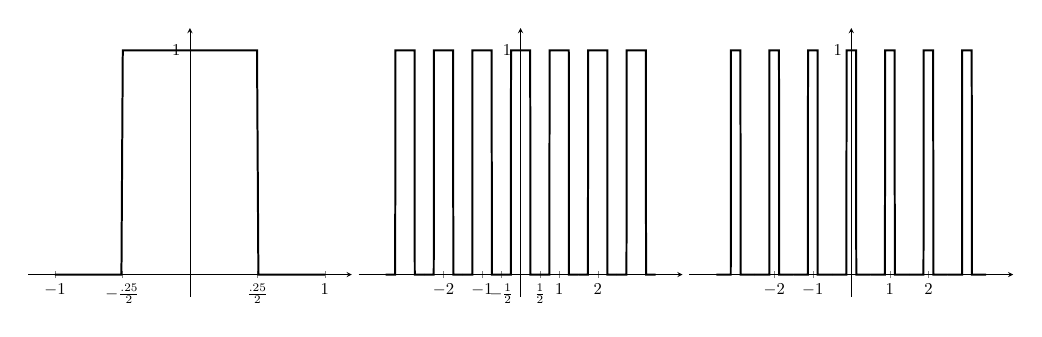
\begin{tikzpicture}[scale=.6]
\begin{scope}\begin{axis}[axis lines=middle,no markers,enlargelimits,xtick={-1,-.5,0,.5,1},xticklabels={$-1$,$-\frac{\tau}{2}$,$0$,$\frac{\tau}{2}$,$1$},ytick={0,1}]
\addplot [very thick,samples=200,domain=-1:1]  {abs(x)<.5?1:0};
\end{axis}\end{scope}
\begin{scope}[xshift=7cm]\begin{axis}[axis lines=middle,no markers,enlargelimits,xtick={-2,-1,-.5,0,.5,1,2},xticklabels={$-2$,$-1$,$-\frac{1}{2}$,0,$\frac{1}{2}$,$1$,$2$},ytick={0,1}]
\def\_tau{.5}
\def\T{1}
\foreach \n in {-3,-2,-1,0,1,2,3}
\addplot [very thick,samples=200,domain=\T*\n-\T/2:\T*\n+\T/2]  {abs(x-\n*\T)<\_tau/2?1:0};
\end{axis}\end{scope}
\begin{scope}[xshift=14cm]\begin{axis}[axis lines=middle,no markers,enlargelimits,xtick={-2,-1,0,1,2},ytick={0,1}]
\def\tau{.25}
\def\T{1}
\foreach \n in {-3,-2,-1,0,1,2,3}
\addplot [very thick,samples=200,domain=\T*\n-\T/2:\T*\n+\T/2]  {abs(x-\n*\T)<\tau/2?1:0};
\end{axis}\end{scope}
\end{tikzpicture}
\end{center}
\caption{Segnale rettangolare e onde quadre con \emph{duty cycle} del 50\% e 25\%}
\end{figure}

\subsection{Delta di Dirac}\index{segnale!impulso}
Il segnale rettangolare $\frac{1}{T} \rect{\frac{1}{T}}$ di base T e altezza 1/T ha area unitaria. Portando al limite $T\to 0$ il rettangolo diventa un impulso. Non una funzione in senso proprio ma una distribuzione integrabile chiamata \keyword[segnale!delta di Dirac|see {impulso}]{delta di Dirac}: \[\delta(t)=\lim\limits_{T\to 0}\frac{1}{T}\rect{\frac{1}{T}}\]

\subsubsection{Proprietà dell'impulso}
\begin{enumerate}
\item il segnale impulso ha area unitaria \[ \intinf{\impulse(t)}{t}=1 \]
\item il segnale impulso è funzione pari \[ \impulse(t)=\impulse(-t) \]
\item estrazione di un campione da un segnale $s(t)$ con un impulso in $t=\tau$ \[ \intinf{s(t)\impulse(t-\tau)}{t}=s(\tau) \]
è equivalente ad un impulso in $\tau$ di area $s(\tau)$
\begin{align*}
 s(t)\impulse(t-\tau)=s(\tau)\impulse(t-\tau) &\implies \\ & \intinf{s(t)\impulse(t-\tau)}{t} =\intinf{s(\tau)\impulse(t-\tau)}{t} = s(\tau)\intinf{\impulse(t-\tau)}{t} = s(\tau)
 \end{align*}
 
\item rappresentazione di un segnale come somma di infiniti impulsi
\[s(t)=\intinf{s(\tau)\impulse(t-\tau)}{\tau}=s(t)\ast\impulse(t)\]
\item derivata dell'impulso (\textsc{doppietto}) $\impulse'(t)$
\[ \intinf{s(t)\impulse'(t-\tau)}{t}=-s'(\tau) \]
\begin{proof}[Dim.]
applico l'integrazione per parti $\int{u \diff v}=u v-\int{v\diff u}$ con $u=s(t) ,\, \diff u=s'(t)\diff t ,\, \diff v=\impulse'(t-\tau)\diff t ,\, v=\impulse(t-\tau)$  a 
\[\intinf{s(t)\impulse'(t-\tau)}{t}= \restrict{s(t)\impulse(t-\tau)}{-\infty}^{+\infty} -\intinf{\impulse(t-\tau)s'(t)}{t}=-s'(\tau)  \]
\end{proof}
\item impulso è derivata del gradino
\[\intinf{\impulse(\tau)}{\tau}=\step(t)  \to \impulse(t)=\deriv{\step(t)}{t} \]
\item scala
\[\impulse(a t+b)=\intinf{s(t)\impulse(a t+b)}{t}\]
applicando le sostituzioni $\begin{cases}x=a t+b \\ t=\frac{x-b}{a}\end{cases}$
\[\intinf{\f{s}{\frac{x-b}{a}}\impulse(x)}{\frac{x}{\abs{a}}}=\frac{1}{\abs{a}}\f{s}{-\frac{b}{a}}\]
\[\intinf{s(t)\frac{1}{\abs{a}}\f{\impulse}{t+\frac{b}{a}}}{t}=\frac{1}{\abs{a}}\f{s}{-\frac{b}{a}}\]
\[\implies\impulse(a t+b)=\frac{1}{\abs{a}}\f{\impulse}{t+\frac{b}{a}} \]

\end{enumerate}

\subsection{Segnale sinusoidale}\index{segnale!sinusoidale}
Il segnale sinusoidale di ampiezza $A$, pulsazione angolare $\omega=2\pi f$, periodo $T=\frac{2\pi}{\omega}$, frequenza $f=\frac{1}{T}$, fase iniziale $\phi$
\[s(t)=A\sen{2\pi f t+\phi} \]

Potenza media 
\[P_m=\frac{1}{T}\intd{-T/2}{T/2}{A^2\Sen^2(2\pi f t+\phi)}{t}= \frac{A^2}{2}\]

infatti essendo $\Sen^2(x)=\frac{1}{2}-\frac{1}{2}\cos{2x}$
\[\begin{split}P_m&=\frac{1}{T}\intd{-T/2}{T/2}{\left(\frac{A^2}{2}-\frac{A^2}{2}\cos{4\pi f t+2\phi}\right)}{t}=\\
&=\restrict{\frac{A^2}{2 T}}{-T/2}^{T/2}-\frac{A^2}{2 T}\underbrace{\intd{-T/2}{T/2}{\cos{4\pi f t+2\phi}}{t}}_{=0}=\frac{A^2}{2}\end{split}\]

Potenza di picco \[P_p=\max\limits_{t} A^2\Sen^2(2\pi f t+\phi)=A^2\]

Fattore di picco \[\frac{P_p}{P_m}=2\]

\subsection{Segnale seno cardinale}\index{segnale!seno cardinale}
\[\sinc{t}=\frac{\sen{\pi t}}{\pi t}\]

\begin{figure}[!ht]
\centering
\subfloat[][$\sinc{t}=\frac{\sen{\pi t}}{\pi t}$]
{\begin{tikzpicture}[scale=.8]
\begin{axis}[axis lines=middle,no markers,enlargelimits,xscale=1.5,xtick={0,1,2,3,4,5,6},ytick={0,1}]
\addplot [very thick,domain=-6:6,samples=100] {sin(pi*x)/(pi*x)};
\end{axis}\end{tikzpicture}} \qquad
\subfloat[][$\sinc{\frac{t}{T}}=\frac{\sen{\frac{\pi t}{T}}}{\frac{\pi t}{T}}$]
{\begin{tikzpicture}[scale=.8]
\begin{axis}[axis lines=middle,no markers,enlargelimits,xscale=1.5,xtick={-9.424,-6.283,-3.141,0,3.141,6.283,9.424},ytick={0,1},xticklabels={$-3T$,$-2T$,$-T$,$0$,$T$,$2T$,$3T$}]
\addplot [very thick,domain=-3.1*pi:3.1*pi,samples=100] {sin(x)/x};
\end{axis}\end{tikzpicture}}
\caption{Segnale seno cardinale}
\label{fig:sinc}
\end{figure}
